\documentclass{beamer}
\usepackage[utf8]{inputenc}
\usepackage[T1]{fontenc}
\usepackage[slovene]{babel}
\usepackage{lmodern}
\usepackage{url}
\usepackage{amsmath}
\usepackage{amsthm}

\theoremstyle{definition}
\newtheorem{definicija}{Definicija}


\title{Nekaj o kompleksni dinamiki}
\author{Beno Učakar}
\date{14. \ 2. \ 2024}
\institute{Fakulteta za matematiko in fiziko}


\usetheme{metropolis}
\usetheme{Darmstadt}
\usecolortheme{spruce}
\usefonttheme{structurebold}
\useoutertheme{infolines}
\beamertemplatenavigationsymbolsempty

\begin{document}


\maketitle

\begin{frame}
    Kompleksna števila lahko enostavno vstavimo v polinom, kaj pa druge funkcije? 
    Za primer si poglejmo, kako izračunamo $e^{i\theta}$ s pomočjo Taylorjeve vrste.
    
    % 3. naloga: okolje za poravnano enačbo
    % začetek okolja
    \begin{align*}
        & e^{i\theta} = ?? \frac{(i\theta)^n}{n!} \\
        & = 1 + i\theta - \frac{\theta^2}{2!} - \frac{i\theta^3}{3!} + \frac{\theta^4}{4!} + \frac{i\theta^5}{5!} + \ldots \\
        &  = \left( 1 - \frac{\theta^2}{2!} + \frac{\theta^4}{4!} - \ldots \right)  
          + i \left(\theta - \frac{\theta^3}{3!} + \frac{\theta^5}{5!} - \ldots \right) \\
        &   = ??.
    \end{align*}
       
    % konec okolja
\end{frame}

\begin{frame}

    % 2. naloga: uporabite okolje definicija in poudarite izraz "večkratnost"
    \begin{definicija}
     Naj bo $f \in O(D)$ in $z_0 \in D$ fiksna točka funkcije $f$.
        Število $\lambda = f'(z_0)$ imenujemo \textbf{večkratnost} funkcije $f$ v točki $z_0$.
    \end{definicija}
   
    
        
    
    % 4. naloga: prelom prosojnice

    \begin{exampleblock}{Glede na $\lambda$ karakteriziramo fiksne točke:}
        % 4. naloga: postopno prikazovanje elementov in manjkajoč izraz
        \begin{enumerate} 
           \onslide<1-> \item $|\lambda| = 0$ je \textbf{super privlačna} fiksna točka.
           \onslide<2-> \item $|\lambda| < 1$ je \textbf{privlačna} fiksna točka.
           \onslide<3-> \item $|\lambda| > 1$ je \textbf{odbojna} fiksna točka.
           \onslide<4-> \item $|\lambda| = 1$: 
                če je $\lambda^n \neq 1$ za vsak ?? je fiksna točka \textbf{iracionalno},
                sicer pa \textbf{racionalno nevtralna}.
        \end{enumerate}
    \end{exampleblock}
\end{frame}

\begin{frame}{Primer Julijeve množice}
    % 5. naloga: naslov prosojnice
    % 
\begin{figure}
    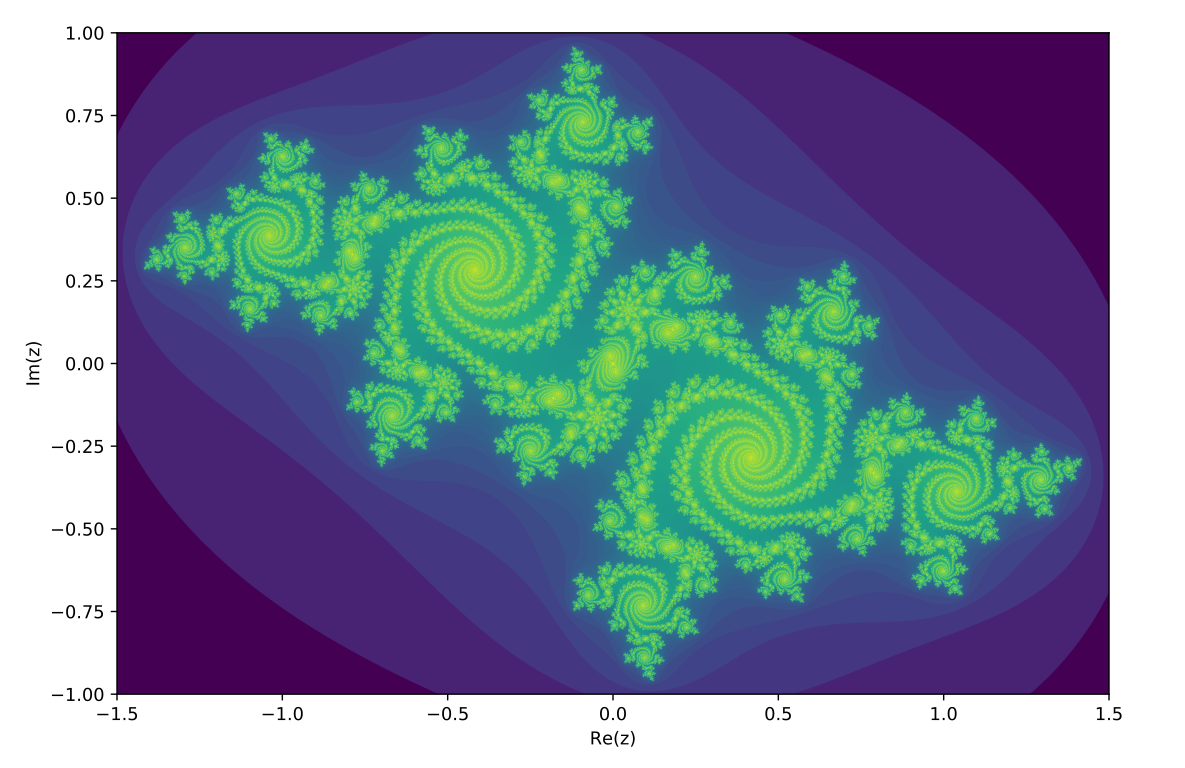
\includegraphics[scale=0.25]{julia_set.png }
\end{figure}
    % 5. naloga: vstavite sliko (potrebujete tudi ustrezen paket)
\end{frame}

\end{document}